\section{Syntax and Semantics}

\begin{frame}[fragile]
\frametitle{What is a program?}

A program is a sequence of one of more statements written to perform a task in a computer:

\begin{example}
\begin{semiverbatim}
x = 21;
y = 21;
z = x + y;
\end{semiverbatim}
\end{example}


\end{frame}

\subsection{Expressions}

\begin{frame}[fragile]
\frametitle{Syntax of expressions}
\framesubtitle{Expressions in Chloe}

\begin{columns}[t]
\column{.45\textwidth}
\begin{semiverbatim}
\textbf{type_synonym} \textit{vname} = string

\textbf{datatype} \textit{exp} = Const \textit{int}
  | Null
  | V      \textit{vname}
  | Plus  \textit{exp} \textit{exp}
  | Subst \textit{exp} \textit{exp}
  | Minus \textit{exp}
  | Div   \textit{exp} \textit{exp}
  | Mod   \textit{exp} \textit{exp}
  | Mult  \textit{exp} \textit{exp}
  | Less  \textit{exp} \textit{exp}
  | Not   \textit{exp}
\end{semiverbatim}
\column{.45\textwidth}
\begin{semiverbatim}
  | And   \textit{exp} \textit{exp}
  | Or    \textit{exp} \textit{exp}
  | Eq    \textit{exp} \textit{exp}
  | New   \textit{exp}
  | Deref \textit{exp}
  | Ref   \textit{lexp}
  | Index \textit{exp} \textit{exp}
and
\textbf{datatype} \textit{lexp} = Deref \textit{exp}
  | Indexl \textit{exp} \textit{exp}
\end{semiverbatim}
\end{columns}


\end{frame}


\begin{frame}[fragile]
\frametitle{Syntax of expressions}
\framesubtitle{Expressions in Chloe}

Why do we have \textit{exp} and \textit{lexp}?
\begin{example}
\begin{semiverbatim}
foo = *bar;
*baz = 1;
\end{semiverbatim}
\end{example}



\end{frame}


\begin{frame}[fragile]
\frametitle{Types}
\framesubtitle{Integers}

Integers are 64 bit length words.
\begin{block}{}
\begin{semiverbatim}
\textbf{type_synonym} int_width = 64
\textbf{type_synonym} int_val = int_width word
\end{semiverbatim}
\end{block}
They have the following bounds:
\begin{block}{}
\begin{semiverbatim}
INT_MIN == - (2^(int_width - 1))
INT_MAX ==  ((2^(int_width - 1)) - 1)
\end{semiverbatim}
\end{block}

\end{frame}

\begin{frame}
\frametitle{Types}
\framesubtitle{Addresses}

An address is a pair representing a block id and an offset.

\begin{semiverbatim}
\textbf{datatype} addr = nat $\times$ int
\end{semiverbatim}

\end{frame}

\begin{frame}[fragile]
\frametitle{Values}
\framesubtitle{}

\begin{semiverbatim}
\textbf{datatype} val = NullVal
             | I \textit{int_val}
             | A \textit{addr}
\end{semiverbatim}

\end{frame}

\begin{frame}[fragile]
\frametitle{Dynamic memory}
\framesubtitle{Layout of the heap}

\begin{semiverbatim}
\textbf{type_synonym} mem = val option list option list
\end{semiverbatim}


\begin{columns}[t]
\column{.45\textwidth}
\begin{block}{Example memory layout}
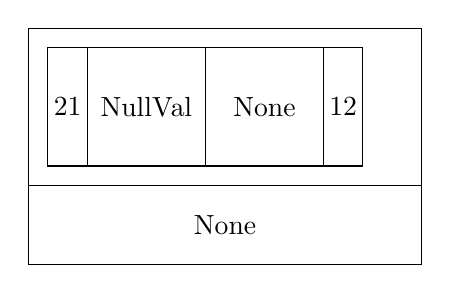
\begin{tikzpicture}
\alert<2>{\draw (0,0) rectangle (5,2);}
\alert<3>{\draw (0,-1) rectangle (5,0) node[midway] {None};}
\alert<4>{\draw (0.25,0.25) rectangle (0.75,1.75) node[midway] {21};}
\draw (0.75,0.25) rectangle (2.25,1.75) node[midway] {NullVal};
\alert<5>{\draw (2.25,0.25) rectangle (3.75,1.75) node[midway] {None};}
\draw (3.75,0.25) rectangle (4.25,1.75) node[midway] {12};
\end{tikzpicture}
\end{block}
\column{.45\textwidth}
\begin{itemize}
\alert<2>{\item{Allocated block}}
\alert<3>{\item{Unallocated block}}
\alert<4>{\item{Initialized cell}}
\alert<5>{\item{Uninitialized cell}}
\end{itemize}
\end{columns}


\end{frame}


\begin{frame}[fragile]
\frametitle{Dynamic Memory}
\framesubtitle{Memory management operations}

\begin{itemize}
\item<1-3>{new\_block :: $val\ \Rightarrow\ mem\ \Rightarrow\ (val\ \times\ mem)$ option}
\item<1,2,4>{free :: $addr\ \Rightarrow\ visible\_state\ \Rightarrow\ visible\_state$ option}
\item<1,2,5>{load :: $addr\ \Rightarrow\ mem\ \Rightarrow\ val$ option}
\item<1,2,6>{store :: $addr\ \Rightarrow\ val\ \Rightarrow\ visible\_state\ \Rightarrow\ visible\_state$ option}
\end{itemize}

\alert<2>{Return types are $\tau$ option, these functions can always fail}

\end{frame}


\begin{frame}[fragile]
\frametitle{Unlimited memory problem}
\framesubtitle{Possible solutions}

Our memory allocation cannot fail because we assume unlimited memory.

\bigskip

However, we have limited resources in a machine.

There are two possible solutions:

\begin{itemize}
\item{Model non-deterministic behavior in our \verb|new_block| function.}
\item{Assume a fixed amount of memory.}
\end{itemize}


\end{frame}


\begin{frame}
\frametitle{Unlimited memory problem}
\framesubtitle{Our solution}

We keep our unlimited memory assumption.

\bigskip
Later in the translation process we wrap C's malloc function in one of our own.

\bigskip
This function checks if a malloc call fails.

\bigskip
If it fails, then the program will be aborted.


\end{frame}


\begin{frame}
\frametitle{Semantics of expressions}
\framesubtitle{What is the meaning of an expression?}

The semantics of an expression is its value and effect on the program state.

\pause
\begin{example}
$21 + 21 = 42$

\pause

$foo + 42 = ?$

\pause

$bar = new (12)$
\end{example}
\pause

We need to know the value of a variable at the time of execution.



\end{frame}


\begin{frame}[fragile]
\frametitle{Semantics of expressions}
\framesubtitle{Valuations}

A valuation is a function that maps a variable name to a value.

\bigskip
\pause

\textbf{type\_synonym} valuation = vname $\Rightarrow$ val option option

\bigskip

\pause
Given a variable name it can yield three results:

\bigskip

\pause
\begin{itemize}
\item{None: undefined variable.}
\pause
\item{Some None: uninitialized variable.}
\pause
\item{Some $v$: initializeid variable holding value $v$.}
\end{itemize}


\end{frame}


\begin{frame}
\frametitle{Semantics of expressions}
\framesubtitle{Visible state}

When we execute a command it can only \textit{see} certain part of the state:

\bigskip
\pause

\textbf{type\_synonym} visible\_state = valuation $\times$ valuation $\times$ mem

\bigskip
\pause
\begin{itemize}
\item{Local variables to the current function}
\pause
\item{Global variables}
\pause
\item{Memory}
\end{itemize}


\end{frame}


\begin{frame}
\frametitle{Semantics of expressions}
\framesubtitle{Evaluation functions eval and eval\_l}

We define functions to compute the values of an expressions:

\bigskip

\textbf{eval} :: exp $\Rightarrow$ visible\_state $\Rightarrow$ (val $\times$ visible\_state) option

\textbf{eval\_l} :: exp $\Rightarrow$ visible\_state $\Rightarrow$ (addr $\times$ visible\_state) option

\bigskip

The evaluation of functions can fail:

\bigskip
\pause

\begin{itemize}
\item{Undefined variables}
\pause
\item{Illegal operands given to the function}
\pause
\item{Trying to access invalid memory}
\pause
\item{Integer overflow}
\pause
\item{Division by zero}
\end{itemize}


\end{frame}


\begin{frame}
\frametitle{Semantics of expressions}
\framesubtitle{Highlights of expression evaluation}

\begin{itemize}
\item{Integer overflow is detected and leads to an erroneous state}
\item{Short-circuit evaluation}
\item{Division and modulo towards zero}
\item{Static scoping of variables}
\end{itemize}


\end{frame}


\subsection{Commands}


\begin{frame}[fragile]
\frametitle{Syntax of commands}
\framesubtitle{Concrete syntax}

\begin{semiverbatim}
com ::= SKIP
     | lexp ::== exp
     | vname ::= exp
     | com ;; com
     | IF exp THEN com ELSE com
     | WHILE exp DO com
     | FREE lexp
     | RETURN exp
     | RETURNV
     | lexp ::== f ( [exp] )
     | vname ::= f ( [exp] )
     | CALL f ( [exp])
\end{semiverbatim}


\end{frame}


\begin{frame}[fragile]
\frametitle{Syntax of commands}
\framesubtitle{Abstract syntax}

\begin{semiverbatim}
\textbf{datatype} com = SKIP
             | Assignl lexp exp
             | Assign  vname exp
             | Seq     com  com
             | If      exp com com
             | While   exp com
             | Free    lexp
             | Return exp
             | Returnv
             | Callfunl lexp fname " exp list"
             | Callfun vname fname " exp list"
             | Callfunv fname " exp list"
\end{semiverbatim}

\end{frame}


\begin{frame}[fragile]
\frametitle{Functions}
\framesubtitle{}

We have functions that return a value and those that do not.

\begin{semiverbatim}
\textbf{record} fun_decl =
  name :: fname
  params :: vname list
  locals :: vname list
  body :: com
\end{semiverbatim}

\bigskip

A function is valid $\Longleftrightarrow$ the function parameters and the local variables have different names

\bigskip

When a function returns a value, this value will be:

\begin{itemize}
\item{Assigned to a location in memory}
\item{Assigned to a variable}
\item{Ignored}
\end{itemize}


\end{frame}


\begin{frame}[fragile]
\frametitle{Programs}

\begin{semiverbatim}
\textbf{record} program =
  name :: fname
  globals :: vname list
  procs :: fun_decl list
\end{semiverbatim}
\pause

\begin{block}{A program is considered valid if:}
\begin{itemize}
\item{The global variable names are different from one another.}
\pause
\item{Function names within a program are different from one another.}
\pause
\item{All function declarations are valid.}
\pause
\item{The main function is defined.}
\pause
\item{None of the variable names or function names in the program is a reserved keyword.}
\pause
\item{Global variables and function names are disjoint.}
\end{itemize}
\end{block}


\end{frame}


\begin{frame}[fragile]
\frametitle{Stack}
\framesubtitle{Return locations and stack frames}

\begin{semiverbatim}
\textbf{datatype} return_loc = \alert<3>{Ar \textit{addr}} | \alert<4>{Vr \textit{vname}} | \alert<5>{Invalid}
\end{semiverbatim}

\pause

A return value of a function can be:
\begin{itemize}
\item<3->{\alert<3>{Assigned to a cell in memory}}
\item<4->{\alert<4>{Assigned to a variable}}
\item<5->{\alert<5>{Ingnored}}
\end{itemize}


\bigskip
\onslide<6->{\textbf{datatype} stack\_frame = com $\times$ valuation $\times$ return\_loc}

\bigskip

\onslide<6>{The execution stack is a list of stack frames.}


\end{frame}


\begin{frame}[fragile]
\frametitle{Stack}
\framesubtitle{Calling convention}

\only<2,4>{
\begin{drawstack}[baseline=(current bounding box.north), scale=0.8]
  \only<2>{
  \startframe
  \cell{x=sum(2,2)}
  \cell{[x$\mapsto$0]}
  \cell{Invalid}
  \finishframe{main}}
  \only<4>{
  \startframe
  \cell{return a+b}
  \cell{[a$\mapsto$2, b$\mapsto$2]}
  \alert<4>{\cell{Invalid}}
  \finishframe{sum}
  \startframe
  \cell{x=sum(2,2)}
  \cell{[x$\mapsto$0]}
  \alert<4>{\cell{x}\only<4>{\cellround{Caller's rloc changes!}}}
  \finishframe{main}
  }
\end{drawstack}
}

\begin{semiverbatim}
\only<1,3>{
int sum(int a; int b){
  return a+b;
}

int main(){
  int x = 0;
  \alert<3>{x = sum(2,2);}
}
}
\end{semiverbatim}


\end{frame}

\subsection{States}

\begin{frame}
\frametitle{Procedure table and States}
\framesubtitle{}

The procedure table maps function names to function declarations:
\bigskip

\textbf{type\_synonym} proc\_table = fname $\rightharpoonup$ fun\_decl
\pause
\bigskip

It is built by pairing every function declaration to its name.

\pause
\bigskip

A state is defined as follows:
\bigskip
\pause

\textbf{type\_synonym} state = stack\_frame list $\times$ valuation $\times$ mem


\end{frame}


\begin{frame}
\frametitle{State}
\framesubtitle{Initial state}

An initial state will be the tuple conaining:

\begin{itemize}
\item{Initial stack: Stack containing the stack frame from the main function}
\item{Initial globals: All variable names mapped to undefined and global variables mapped to uninitialized}
\item{Initial memory: Empty memory}
\end{itemize}


\end{frame}


\subsection{Small-step semantics}


\begin{frame}[fragile]
\frametitle{Control Flow Graph}
\framesubtitle{What is a CFG?}

Graph representation covering the different paths that a program can take during its execution.


\begin{figure}
\centering
\tikzstyle{cfg_node} = [circle, draw, fill=uablue25, 
    text width=2em, text centered, minimum height=1em, line width=1pt ]
\tikzstyle{line} = [line width=1pt, -triangle 45]
\tikzstyle{alert} = [text=uared100, fill=uared25, draw=uared100]
\tikzstyle{alert_pp} = [text=uared100]
\tikzstyle{dim} = [text=uablue25, fill=uablue5, draw=uablue25]

\begin{tikzpicture}[node distance=1.5cm, auto]
    % Place nodes
    \node [cfg_node,onslide=<2>{alert}] (c1) {$c_1$};
    \node [cfg_node,onslide=<2>{alert}] (c2) [right of=c1, node distance=3cm] {$c_2$};
    \node [onslide=<6>{alert_pp}](pp) [above left of=c1, node distance=1.5cm] {program pointer};
    %\node [block,onslide=<2->{dim}] (client) {Web Client};
    %\node [block,onslide=<2->{dim}] (python) [right of=client, node distance=3cm] {Python Service};
    %\node [block,onslide=<2->{dim}] (wavefront) [right of=python, node distance=3cm] {Wavefront};
    %\node [block,onslide=<2->{dim}] (AMCL) [above of=wavefront] {AMCL};
    %\node [block,temporal=<2>{}{alert}{dim}] (VFH) [below of=wavefront] {VFH};
    %\node [block,onslide=<2->{dim}] (laser) [above right=0.5cm and 1.2cm of AMCL] {Laser};
    %\node [block,onslide=<2->{dim}] (dash7) [right of=AMCL, node distance=3cm] {DASH7};
    %\node [block,onslide=<2->{dim},temporal=<3>{}{alert}{dim}] (robot) [right of=wavefront, node distance=3cm] {Robot};
    % Draw edges
    \draw [line,onslide=<3-5>{alert}] (c1) node[above right of=c1, node distance=1.25cm] {(en, tr)} -> (c2);
    \draw [line,onslide=<6>{alert}] (pp) -> (c1);
    %\draw [line] (client.east) -> (python.west);
    %\draw [line] (python) -> (client);
    %\draw [line] (python) -- (wavefront);
    %\draw [line] (AMCL) -- (wavefront);
    %\draw [line] (AMCL) edge[out=180,in=90] (python);
    %\draw [line] (python) edge[out=270,in=180] (VFH);
    %\draw [line] (wavefront) -- (VFH);
    %\draw [line] (laser) -> (AMCL);
    %\draw [line] (dash7) -> (AMCL);
    %\draw [line] (robot) -> (AMCL);
    %\draw [line] (VFH) edge[out=0,in=270] (robot);
\end{tikzpicture}
\end{figure}


\begin{itemize}
\item<2->{The nodes in our CFG are commands}
\item<3->{The edges in our CFG are annotated with two functions that depend on the program state}
  \begin{itemize}
  \item<4->{The first one indicates whether a an edge can be followed or not}
  \item<5->{The second one indicates how the state is tranformed by following the edge}
  \end{itemize}
 \item<6->{We have a current location, which is a program pointer to the current node}
\end{itemize}


\end{frame}


\begin{frame}
\frametitle{Control Flow Graph}
\framesubtitle{Enabled functions}

\begin{figure}[fragile]
\centering
\tikzstyle{cfg_node} = [circle, draw, fill=uablue25, 
    text width=2em, text centered, minimum height=1em, line width=1pt ]
\tikzstyle{cfg_big_node} = [circle, draw, fill=uablue25, 
    text width=4.5em, text centered, minimum height=2.25em, line width=1pt ]
\tikzstyle{line} = [line width=1pt, -triangle 45]
\tikzstyle{alert} = [text=uared100, fill=uared25, draw=uared100]
\tikzstyle{alert_pp} = [text=uared100]
\tikzstyle{dim} = [text=uablue25, fill=uablue5, draw=uablue25]

\begin{block}{}
\textbf{type\_synonym} enabled = state $\rightharpoonup$ bool
\end{block}

\bigskip


\begin{tikzpicture}[node distance=1.5cm, auto]
    % Place nodes
    \node [cfg_big_node,onslide=<1>{dim},onslide=<2-3>{alert}] (if) {IF $b$ THEN $c_1$ ELSE $c_2$};
    \node [cfg_node,onslide=<1>{dim},onslide=<2>{alert}] (c1) [right of=if, node distance=4cm] {$c_1$};
    \node [cfg_node,onslide=<1-2>{dim},onslide=<3>{alert}] (c2) [left of=if, node distance=4cm] {$c_2$};
    %\node [block,onslide=<2->{dim}] (client) {Web Client};
    %\node [block,onslide=<2->{dim}] (python) [right of=client, node distance=3cm] {Python Service};
    %\node [block,onslide=<2->{dim}] (wavefront) [right of=python, node distance=3cm] {Wavefront};
    %\node [block,onslide=<2->{dim}] (AMCL) [above of=wavefront] {AMCL};
    %\node [block,temporal=<2>{}{alert}{dim}] (VFH) [below of=wavefront] {VFH};
    %\node [block,onslide=<2->{dim}] (laser) [above right=0.5cm and 1.2cm of AMCL] {Laser};
    %\node [block,onslide=<2->{dim}] (dash7) [right of=AMCL, node distance=3cm] {DASH7};
    %\node [block,onslide=<2->{dim},temporal=<3>{}{alert}{dim}] (robot) [right of=wavefront, node distance=3cm] {Robot};
    % Draw edges
    \draw [line,onslide=<2>{alert}] (if) node[above left of=c1, node distance=1.5cm] {(en\_pos, tr)} -> (c1);
    \draw [line,onslide=<3>{alert}] (if) node[above right of=c2, node distance=1.5cm] {(en\_neg, tr)} -> (c2);
    %\draw [line] (client.east) -> (python.west);
    %\draw [line] (python) -> (client);
    %\draw [line] (python) -- (wavefront);
    %\draw [line] (AMCL) -- (wavefront);
    %\draw [line] (AMCL) edge[out=180,in=90] (python);
    %\draw [line] (python) edge[out=270,in=180] (VFH);
    %\draw [line] (wavefront) -- (VFH);
    %\draw [line] (laser) -> (AMCL);
    %\draw [line] (dash7) -> (AMCL);
    %\draw [line] (robot) -> (AMCL);
    %\draw [line] (VFH) edge[out=0,in=270] (robot);
\end{tikzpicture}
\end{figure}

\only<1>{This function indicates whether a state is able to continue its execution.

It is a partial function, therefore it might fail.}

\only<2>{When the evaluation of the condition b yields true, we follow the edge that leads to $c_1$.}

\only<3>{When the evaluation of the condition b yields false, we follow the edge that leads to $c_2$.}

\only<4>{Depending on the result of the enabled function we decide which edge to take.}

\only<5>{There will always be an enabled edge that can be followed.}

\end{frame}


\begin{frame}
\frametitle{Control Flow Graph}
\framesubtitle{Transformer functions}

\begin{block}{}
\textbf{type\_synonym} transformer = state $\rightharpoonup$ state
\end{block}
\bigskip

This function transforms a state to a new one depending on the edge followed.

\bigskip

It is a partial function, it fails when an error is encountered in the transformation.

\bigskip

This is the function that will update the state with the resulting state every time an edge is followed.



\end{frame}


\begin{frame}
\frametitle{Control Flow Graph}
\framesubtitle{How do our transformer functions behave?}

\only<1>{We have a set of functions that will take the neccessary parameters to yield an appropiate transformer function for each command in Chloe.}

\pause
\begin{itemize}
\item\only<2->{{\textbf{tr\_id} :: transformer where tr\_id $\equiv$ Some}}
\item\only<3->{{\textbf{tr\_assign} :: vname $\Rightarrow$ exp $\Rightarrow$ transformer}}
\item\only<4->{{\textbf{tr\_assignl} :: lexp $\Rightarrow$ exp $\Rightarrow$ transformer}}
\item\only<5->{{\textbf{tr\_eval} :: exp $\Rightarrow$ transformer}}
\item\only<6->{{\textbf{tr\_free} :: lexp $\Rightarrow$ transformer}}
\item\only<7->{{\textbf{call\_function} :: proc\_table $\Rightarrow$ fname $\Rightarrow$ exp list $\Rightarrow$ transformer}}
\item\only<8->{{\textbf{tr\_callfunl} :: proc\_table $\Rightarrow$ lexp $\Rightarrow$ fname $\Rightarrow$ exp list $\Rightarrow$ transformer}}
\item\only<9->{{\textbf{tr\_callfun} :: proc\_table $\Rightarrow$ vname $\Rightarrow$ fname $\Rightarrow$ exp list $\Rightarrow$ transformer}}
\item\only<10->{{\textbf{tr\_callfunv} :: proc\_table $\Rightarrow$ fname $\Rightarrow$ exp list $\Rightarrow$ transformer}}
\item\only<11->{{\textbf{tr\_return} :: exp $\Rightarrow$ transformer}}
\item\only<12->{{\textbf{tr\_return\_void} :: transformer}}
\end{itemize}

\end{frame}


\begin{frame}[fragile]
\frametitle{Control Flow Graph}
\framesubtitle{... with a stack}

\begin{figure}
\centering
\tikzstyle{cfg_node} = [circle, draw, fill=uablue25, 
    text width=1em, text centered, minimum height=1em, line width=1pt ]
\tikzstyle{line} = [line width=1pt, -triangle 45]
\tikzstyle{alert} = [text=uared100, fill=uared25, draw=uared100]
\tikzstyle{alert_pp} = [text=uared100]
\tikzstyle{dim} = [text=uablue25, fill=uablue5, draw=uablue25]

\begin{tikzpicture}[node distance=1.5cm, auto, baseline=(current bounding box.north)]
    % Place nodes
    \node [cfg_node] (c1) {$f()$};
    \node [cfg_node] (c2) [right of=c1, node distance=3cm] {$c_2$};
    \node (pp) [above left of=c1, node distance=1.5cm] {program pointer};
    \node (pp3) [above left of=c2, node distance=1.5cm] {program pointer};

    \node [cfg_node] (c3) [below of=c1, node distance=3cm] {$c_3$};
    \node (pp2) [above left of=c3, node distance=1.5cm] {f()};
    \node [cfg_node] (c4) [right of=c3, node distance=1.5cm] {$c_4$};
    \node [cfg_node] (c5) [right of=c4, node distance=1.5cm] {$c_5$};
    % Draw edges
    \draw [line] (c1) -> (c2);
    \draw [line] (c3) -> (c4);
    \draw [line] (c4) -> (c5);
    \draw [line,onslide=<2->{dim}] (pp) -> (c1);
    \draw [line,onslide=<2>{alert},onslide=<3->{dim},onslide=<1>{dim}] (pp3) -> (c2);
    \draw [line,onslide=<3>{alert},onslide=<1-2>{dim}] (pp2) -> (c3);
\end{tikzpicture}
\end{figure}

\begin{tikzpicture}[stack/.style={rectangle split, rectangle split parts=#1,draw, anchor=center}, baseline=(current bounding box.north)]
\only<2>{
\node[stack=3]{
\nodepart{three}$c_2$
};
}

\only<3->{
\node[stack=3]{
\nodepart{two}$f()$
\nodepart{three}$c_2$
};
}
\end{tikzpicture}


\end{frame}


\begin{frame}[fragile]
\frametitle{Control Flow Graph}
\framesubtitle{Rules}

\textbf{type\_synonym} cfg\_label = enabled $\times$ transformer

\bigskip

\textbf{inductive} cfg :: com $\Rightarrow$ cfg\_label $\Rightarrow$ com $\Rightarrow$ bool

\begin{itemize}
\item{Assign: \textbf{cfg} ($x$ ::= $a$) (en\_always,tr\_assign $x$ $a$) SKIP}
\item{Assignl: \textbf{cfg} ($x$ ::==  $a$) (en\_always,tr\_assignl $x$ $a$) SKIP}
\item{Seq1: \textbf{cfg} (SKIP;; $c_{2}$) (en\_always, tr\_id) $c_{2}$}
\item{Seq2: $[\![$\textbf{cfg} $c_{1}$ $a$ $c_{1}'$ $]\!]$ $\Longrightarrow$ \textbf{cfg} ($c_{1}$;; $c_{2}$) $a$ ($c_{1}'$;; $c_{2}$)}
\item{IfTrue: \textbf{cfg} (IF $b$ THEN $c_{1}$ ELSE $c_{2}$) (en\_pos $b$, tr\_eval $b$) $c_{1}$}
\item{IfFalse: \textbf{cfg} (IF $b$ THEN $c_{1}$ ELSE $c_{2}$) (en\_neg $b$, tr\_eval $b$) $c_{2}$}
\item{While: \textbf{cfg} (WHILE $b$ DO $c$) (en\_always, tr\_id)
  (IF $b$ THEN $c$;; WHILE $b$ DO $c$ ELSE SKIP)}
\item{Free: \textbf{cfg} (FREE $x$) (en\_always, tr\_free $x$) SKIP}
\end{itemize}

\end{frame}


\begin{frame}[fragile]
\frametitle{Control Flow Graph}
\framesubtitle{Rules}

\begin{itemize}
\item{Return: \textbf{cfg} (Return $a$) (en\_always, tr\_return $a$) SKIP}
\item{Returnv: \textbf{cfg} Returnv (en\_always, tr\_return\_void) SKIP}

\item{Callfunl: \textbf{cfg} (Callfunl $e$ $f$ params)
  (en\_always, tr\_callfunl proc\_table $e$ $f$ params) SKIP}
\item{Callfun: \textbf{cfg} (Callfun $x$ $f$ params)
  (en\_always, tr\_callfun proc\_table $x$ $f$ params) SKIP}
\item{Callfunv: \textbf{cfg} (Callfunv $f$ params)
  (en\_always, tr\_callfunv proc\_table $f$ params) SKIP}
\end{itemize}

\end{frame}


\begin{frame}
\frametitle{Small-step semantics}
\framesubtitle{}

Why a small-step semantics?
\bigskip
\pause

We want talk about intermediate states and differentiate betwwen non-termination and getting stuck.

\bigskip
\pause


\begin{block}{Our small-step semantics is defined over states:}
\textbf{inductive} small\_step :: state $\Rightarrow$ state option $\Rightarrow$ bool
\bigskip

$s\ \rightarrow\ s_2$

$\equiv$

``We take a small step from $s$ to $s_2$''
\end{block}


\end{frame}


\begin{frame}
\frametitle{Small-step semantics}
\framesubtitle{When can a step be taken?}

A step from $s$ to $s_2$ can be taken when:
\begin{itemize}
\item{Regular step:}
\begin{itemize}
\item{Non-empty stack}
\item{CFG edge between $c_1$ and $c_2$}
\item{The command at the top of the stack is $c_1$}
\item{Applying the enabled function yields True}
\item{Applying the transformer function over $s$ yields $s_2$}
\end{itemize}
\item{Return step from a function without return value:}
\begin{itemize}
\item{Non-empty stack}
\item{The command at the top of the stack is SKIP}
\item{Applying the transformer function tr\_return\_void over $s$ yields $s_2$}
\end{itemize}
\end{itemize}

\end{frame}


\begin{frame}
\frametitle{Small-step semantics}
\framesubtitle{When does taking a step fail?}

When there is an erroneous execution, we take a step from $s$ to None:
\begin{itemize}
\item{Regular step:}
\begin{itemize}
\item{Non-empty stack}
\item{CFG edge between $c_1$ and $c_2$}
\item{The command at the top of the stack is $c_1$}
\item{The enabled function or the transformer function yield None}
\end{itemize}
\item{Return step from a function without return value:}
\begin{itemize}
\item{Non-empty stack}
\item{The command at the top of the stack is SKIP}
\item{Applying the transformer function tr\_return\_void yields None.}
\end{itemize}
\end{itemize}


\end{frame}


%\begin{frame}
%\frametitle{Small-step semantics}
%\framesubtitle{How do we take several steps?}
%
%We lift the definition of small\_step over to states:
%
%\bigskip
%\textbf{inductive} small\_step' :: state option $\Rightarrow$ state option $\Rightarrow$ bool
%\bigskip
%\pause
%
%To take several steps we then use the reflexive transitive closure over small\_step':
%
%\bigskip
%\textbf{inductive} small\_step' :: state option $\Rightarrow$ state option $\Rightarrow$ bool
%\bigskip
%
%$s\ \rightarrow*\ s_2$
%
%$\equiv$
%
%``We take one or more small steps from $s$ to $s_2$''
%
%
%
%\end{frame}


\subsection{Interpreter}


\begin{frame}
\frametitle{Interpreter}
\framesubtitle{Execution of a program}

A single step is executed by applying the correspoding transformer function to a state and updating the command at the top of the stack.
\bigskip
\pause

Our semantics is deterministic, which enables us to write an interpreter for it.
\bigskip
\pause

\begin{block}{Interpretation of a program:}
While a final state has not been reached yet, execute a single step.
\end{block}

\pause

\begin{block}{Execution of a program:}
Assert that a program is valid.

If it is, proceed to interpret it.
\end{block}

\bigskip

The interpreter will either return a final state or a None, which indicates an erroneous execution.

\end{frame}
